\section{ŠUM ODPORU, ŠUM MOS TRANZISTORU }
Základní charakteristiky a rovnice pro výpočet, vliv parametrů odporů a MOS, ekvivalentní vstupní šum MOS tranzistoru, ekvivalentní vstupní šum MOS zesilovače

\subsection{Šum odporu}
Šum odporu se dá definovat pomocí zdroje šumového napětí, který je v sérii s daným
odporem:
\begin{equation}
v_{nR}=\sqrt{4*k*T*R}
\end{equation}

\begin{figure}[h]
   \begin{center}
     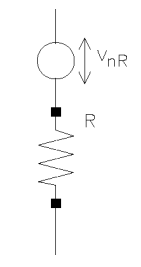
\includegraphics[scale=0.5]{images/sumR.png}
   \end{center}
   \caption{Šumové napětí odporu}
\end{figure}

Nebo pomocí proudového zdroje, který je připojen paralelně k danému odporu:
\begin{equation}
i_{nR}=\frac{V_{nR}}{R}=\frac{\sqrt{4kT*R}}{R}=\sqrt{\frac{4kT}{R}}
\end{equation}

\begin{figure}[h]
   \begin{center}
     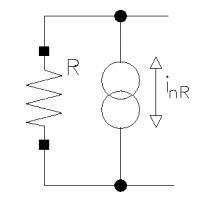
\includegraphics[scale=0.5]{images/sumRI.png}
   \end{center}
   \caption{Šumový proud odporu}
\end{figure}

\subsection{Šum MOS}
Šumové parametry MOS tranzistoru jsou definovány jediným šumovým zdrojem – proudovým šumem i\textsubscript{nd}, který se modeluje jako zdroj proudu i\textsubscript{nd} paralelně k MOS tranzistoru.

\begin{figure}[h]
   \begin{center}
     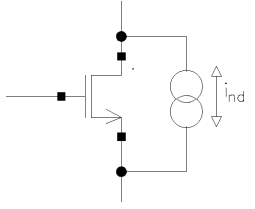
\includegraphics[scale=0.5]{images/sumMOS.png}
   \end{center}
   \caption{Šumový proud MOS tranzistoru}
\end{figure}
\begin{equation}
i_{nd}=\sqrt{4kT*g_{CH}}
\end{equation}
 kde g\textsubscript{CH} je vodivost kanálu.
 
Naprosto klíčovým poznatkem je, že g\textsubscript{CH} $\approx$ g\textsubscript{m} , tedy že vodivost kanálu je dána transkonduktancí g\textsubscript{m}:
\begin{equation}
i_{nd}=\sqrt{4kT*g_{m}}
\end{equation}
\subsection*{Ekvivalentní vstupní šum}
Z praktických důvodů je někdy užitečné převést šumový proud na vstup (gate) jako vstupní
šumové napětí v\textsubscript{ni}:
\begin{equation}
v_{ni}=\sqrt{\frac{4kT}{g_{m}}}
\end{equation}
\begin{equation}
gm = \sqrt{2*I_{d}*kp*\frac{W}{L}}
\end{equation}

\begin{figure}[h]
   \begin{center}
     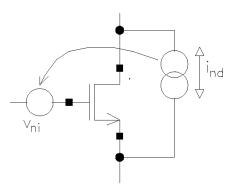
\includegraphics[scale=0.5]{images/sumMOSv.png}
   \end{center}
   \caption{Přepočet šumového proudu i\textsubscript{nd} do šumového napětí v\textsubscript{ni}}
\end{figure}

Šum MOS tranzistoru pro silnou inverzi:
\begin{equation}
v_{ni}=\sqrt{\frac{4kT}{g_{m}}}
\end{equation}
Šum MOS tranzistoru pro slabou inverzi:
\begin{equation}
v_{ni}=\sqrt{\frac{4kT}{g_{m}}}
\end{equation}
\begin{equation}
gm = \frac{I_{d}}{n*U_{T}}
\end{equation}
\begin{equation}
v_{ni}=2*U_{T}*\sqrt{\frac{n*q}{I_{d}}}
\end{equation}

Kmitočet lomu 1/f šumu je pro běžné mosové tranzistory poměrně vysoký (stovky Hz až
jednotky kHz), proto nejsou mosové tranzistory příliš vhodné pro nízkošumové aplikace
v oblasti velmi nízkých kmitočtů. Kmitočet lomu 1/f šumu je ovlivněn i rozměry tranzistoru.

\subsection{Ekvivalentní vstupní šum MOS zesilovače}
\begin{figure}[h]
   \begin{center}
     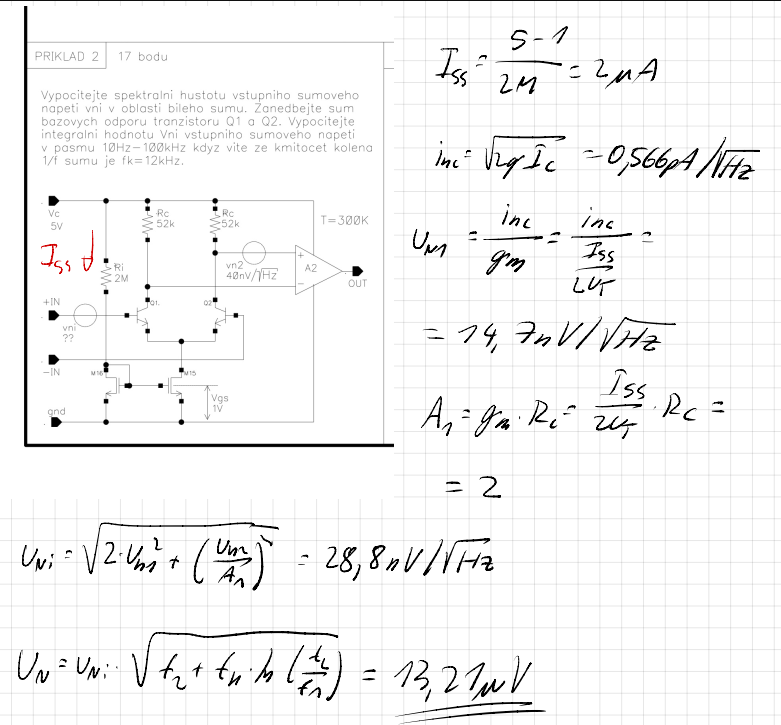
\includegraphics[scale=0.7]{images/vstupMOS1.png}
   \end{center}
   \caption{Ekvivalentní vstupní šum MOS zesilovače}
\end{figure}

\begin{figure}[h]
   \begin{center}
     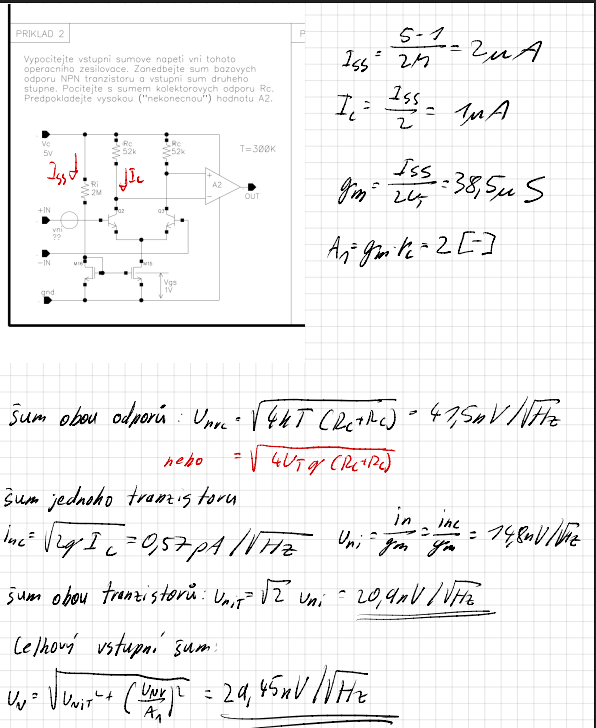
\includegraphics[scale=0.7]{images/vstupMOS2.png}
   \end{center}
   \caption{Ekvivalentní vstupní šum MOS zesilovače}
\end{figure}



